%%%%% Please set the path to 'beamer' directory in your environment %%%%%
\newcommand{\beamerDir}[0]{/mnt/c/Users/atsushi/Documents/workspace/env/Beamer/beamer/beamer/}


%%%%% Load setting %%%%%
\documentclass[aspectratio=169, dvipdfmx, 12pt, compress]{beamer}% dvipdfmxしたい

%%%%% Packages %%%%%
\usepackage{bxdpx-beamer}% dvipdfmxなので必要
\usepackage{pxjahyper}% 日本語で'しおり'したい
\usepackage{tikz}
\usepackage{tcolorbox}
\usetikzlibrary{shapes}
\usepackage{xcolor}
\usepackage[absolute,overlay]{textpos}
\usepackage{adjustbox}
\usepackage{caption}
\usepackage{ifthen}


%%%%% Settings %%%%%
\usetheme[sectionpage=progressbar, subsectionpage=progressbar]{metropolis}
% block style
\metroset{block=fill}
% space between line
\renewcommand{\baselinestretch}{1.3}
% space between item
\newlength{\wideitemsep}
\setlength{\wideitemsep}{0.9\itemsep}
% \addtolength{\wideitemsep}{1.0pt} <- more space
\let\olditem\item
\renewcommand{\item}{\setlength{\itemsep}{\wideitemsep}\olditem}
% frame title
\definecolor{coolblack}{rgb}{0.0, 0.18, 0.39}
\setbeamercolor{frametitle}{bg=coolblack!90,fg=white}
\setbeamerfont{frametitle}{size=\large}
\addtobeamertemplate{frametitle}{}{\vspace{-1em}}
\makeatletter
\setlength{\metropolis@frametitle@padding}{1.4ex}% <- default 2.2 ex
% foot line
\addtobeamertemplate{footline}{}{\vspace{-1em}}
% normal text color
\setbeamercolor{normal text}{fg=black!80}
% progress bar
\definecolor{lightgray}{rgb}{0.83, 0.83, 0.83}
\setbeamercolor{progress bar}{bg=lightgray, fg=coolblack}
\setbeamersize{text margin left=15pt, text margin right=15pt}
% equation font
\usefonttheme{professionalfonts}
% Change standard block width
\addtobeamertemplate{block begin}{%
    \centering
    \begin{columns}\begin{column}{0.9\textwidth}
            \centering
            }{}
            \addtobeamertemplate{block end}{}{\end{column}\end{columns}}
% Change alert block width
\addtobeamertemplate{block alerted begin}{%
    \centering
    \begin{columns}\begin{column}{0.9\textwidth}
            \centering
            }{}
            \addtobeamertemplate{block alerted end}{}{\end{column}\end{columns}}
% Change example block width
\addtobeamertemplate{block example begin}{%
    \centering
    \begin{columns}\begin{column}{0.9\textwidth}
            \centering
            }{}
            \addtobeamertemplate{block example end}{}{\end{column}\end{columns}}
% Itemize color
\setbeamertemplate{itemize item}{\color{black}\scriptsize$\blacksquare$}
\setbeamertemplate{itemize subitem}{\color{black}\scriptsize$-$}
% Simplification  color
\definecolor{cobalt}{rgb}{0.0, 0.28, 0.67}
\setbeamercolor{block title example}{fg=black!80,bg=cobalt!35}
\setbeamercolor{block body example}{fg=black,bg=cobalt!15}
% Definition
\BeforeBeginEnvironment{definition}{
    \setbeamercolor{block title}{use=alerted text, bg=alerted text.fg!70,fg=white}
    \setbeamercolor{block body}{use=alerted text, bg=alerted text.fg!20}
}
\AfterEndEnvironment{definition}{% return to default
    \setbeamercolor{block title}{use=structure,fg=structure.fg,bg=structure.fg!20!bg}
    \setbeamercolor{block body}{parent=normal text,use=block title,bg=block title.bg!50!bg, fg=black}
}
% Theorem
\definecolor{seagreen}{rgb}{0.18, 0.55, 0.34}
\setbeamertemplate{theorems}[numbered]
\BeforeBeginEnvironment{theorem}{
    \setbeamercolor{block title}{fg=black!80,bg=seagreen!40}
    \setbeamercolor{block body}{fg=black,bg=seagreen!15}
}
\AfterEndEnvironment{theorem}{% return to default
    \setbeamercolor{block title}{use=structure,fg=structure.fg,bg=structure.fg!20!bg}
    \setbeamercolor{block body}{parent=normal text,use=block title,bg=block title.bg!50!bg, fg=black}
}
% Lemma
\undef{\lemma}
\newtheorem{lemma}{\translate{Lemma}}
\BeforeBeginEnvironment{lemma}{
    \setbeamercolor{block title}{fg=black!80,bg=seagreen!20}
    \setbeamercolor{block body}{fg=black,bg=seagreen!10}
}
\AfterEndEnvironment{lemma}{% return to default
    \setbeamercolor{block title}{use=structure,fg=structure.fg!80,bg=structure.fg!20!bg}
    \setbeamercolor{block body}{parent=normal text,use=block title,bg=block title.bg!50!bg, fg=black}
}


%%%%% Original Command %%%%%
\newcommand{\subt}[1]{\vspace{-2mm}{\fontsize{10pt}{0cm}\selectfont \textcolor{lightgray}{#1}}\vspace{-1mm}}
\newcommand{\lastpage}[0]{\begin{frame}\begin{textblock*}{1.0\linewidth}(0pt, 50pt)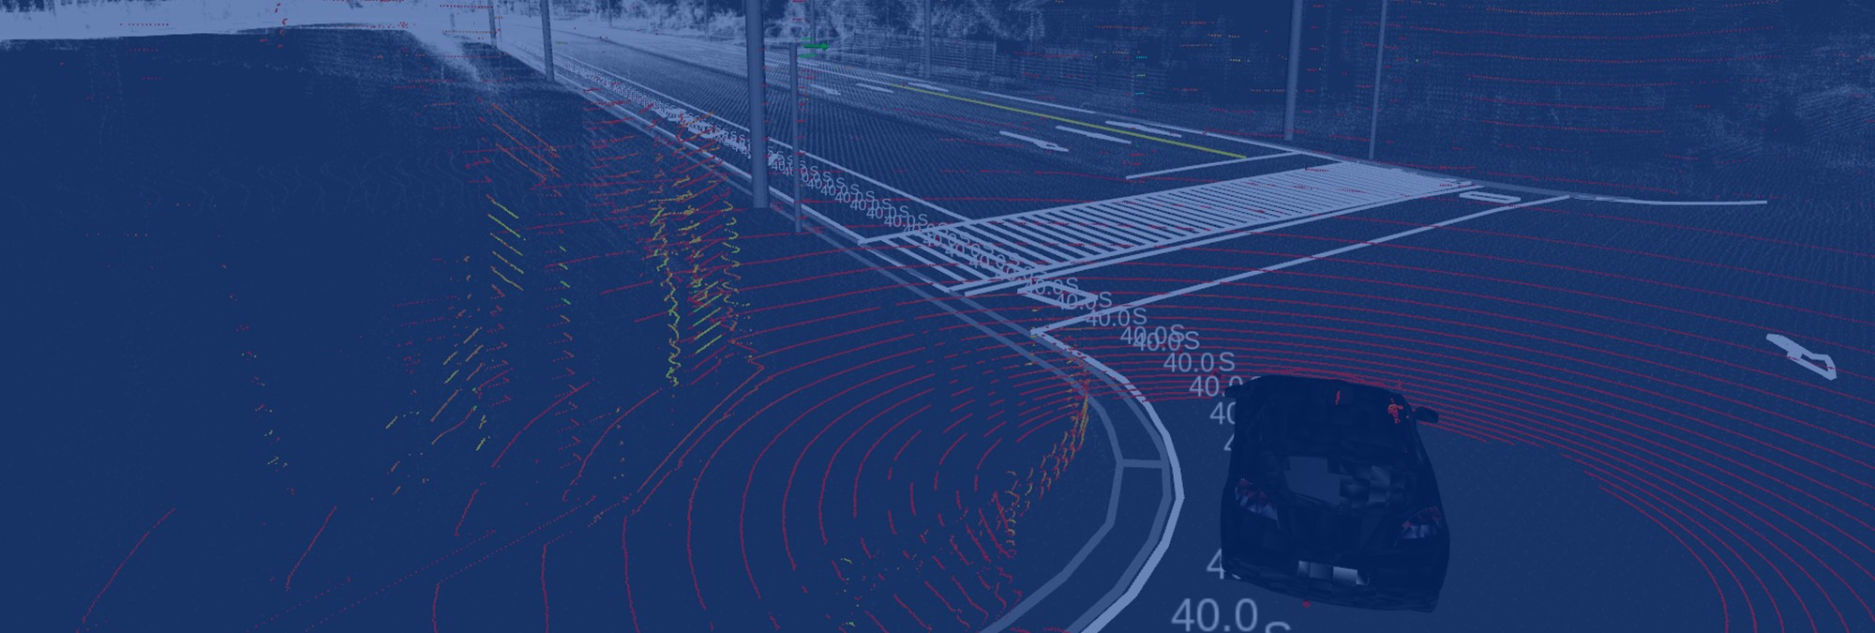
\includegraphics[scale=0.512]{\beamerDir/master_figure/last.pdf}\end{textblock*}\end{frame}}
\newcommand{\todo}[1]{\al{\LARGE\textbf{TODO:} #1}}
\newcommand{\headerheight}[0]{5mm}
\newcommand{\footerheight}[0]{5mm}
\newcommand{\slideheight}[0]{\textheight-\headerheight-\footerheight}
\newcommand{\tabml}[1]{\hspace{-2.1mm}\begin{tabular}{l} #1 \end{tabular}}
\newcommand{\al}[1]{\alert{#1}}
\newcommand{\argempty}[0]{}
\newcommand{\onlyslide}[1]{
    \vspace{\headerheight}
    \begin{minipage}[c][\slideheight][c]{\textwidth}
        #1
    \end{minipage}
}
\newcommand{\onlyimage}[1]{
    \onlyslide{
        \centering
        \begin{columns}
            \begin{column}{\textwidth}
                \centering
                \adjustbox{max width=\textwidth, max height=\slideheight}{
                    \includegraphics{#1}
                }
            \end{column}
        \end{columns}
    }
}
% fit image
\newlength\fitimageht
\newlength\fitotherht
\newsavebox\fitimagebox
\newcommand{\fitimage}[2]{%
    \sbox\fitimagebox{%
        \parbox{\textwidth}{%
            #1\par
        }%
    }%
    \settototalheight{\fitotherht}{%
        \usebox\fitimagebox
    }%
    \setlength\fitimageht{\textheight}%
    \addtolength\fitimageht{-\fitotherht-\headerheight-\footerheight-1\baselineskip}%
    \vspace{\headerheight}
    #1\par
    \centering
    \includegraphics[width=\textwidth,height=\fitimageht,keepaspectratio]{#2}
}
% Simplification
\newcommand{\assume}[1]{
    \begin{exampleblock}{Simplification }
        #1
    \end{exampleblock}
}
% Re-post
\setbeamercolor{RepostBox}{fg=black!50, bg=coolblack!10}
\newcommand{\repost}[1]{
    \vspace{2mm}
    \centering
    \begin{columns}
        \begin{column}{0.86\textwidth}
            \begin{beamercolorbox}[wd=\textwidth, sep=2pt, rounded=true, shadow=true]{RepostBox}
                \begin{tabular}{|p{0.95\textwidth}}
                    {\fontsize{10pt}{10pt}#1}
                \end{tabular}
            \end{beamercolorbox}
        \end{column}
    \end{columns}
}

% equation ballon
\tcbset{
    framebox/.style={
            enhanced,
            boxsep=0pt,       % 箱の上下左右の余白を指定
            colback=white,
            boxrule=1pt,
            colframe=#1
        },
    framebox/.default=red
}
\newcommand{\upbln}[3]{
    \tcboxmath[
        framebox=#2,
        top=0.5ex,bottom=0.5ex,    % 箱の上下の余白を指定
        left=0.5ex,right=0.5ex,    % 箱の左右の余白を指定
        overlay={
                \node[
                    above,
                    rectangle callout,                         % nodeを吹き出しの形に
                    callout absolute pointer={(frame.north)},  % 吹き出しの先端を絶対的に指定
                    fill=#2!20
                ] at ([yshift=2ex]frame.north) {\footnotesize#3};
            }
    ]{#1}
}
\newcommand{\lwbln}[3]{
    \tcboxmath[
        framebox=#2,
        top=0.5ex,bottom=0.5ex,    % 箱の上下の余白を指定
        left=0.5ex,right=0.5ex,    % 箱の左右の余白を指定
        overlay={
                \node[
                    below,
                    rectangle callout,                         % nodeを吹き出しの形に
                    callout absolute pointer={(frame.south)},  % 吹き出しの先端を絶対的に指定
                    fill=#2!20
                ] at ([yshift=-2ex]frame.south) {\footnotesize#3};
            }
    ]{#1}
}
\tcbuselibrary{theorems,skins}



%%%%% Mode %%%%%
% \newcommand{\forme}[1]{#1}
\newcommand{\forme}[1]{}


%%%%% Front Cover %%%%%
\title{Timing-Anomaly Free Dynamic Scheduling of Periodic DAG Tasks with Non-Preemptive}
\subtitle{IEEE International Conference on Embedded and Real-Time Computing Systems and Applications (RTCSA), 2021}
\author{矢野 篤志}
% \date{\today}
\institute[EMBIV]{EMBIV}
\logo{\begin{textblock*}{0.1\linewidth}(2pt, 237pt)
\includegraphics[scale=0.4]{\beamerDir/master_figure/Emb_logo.pdf}\end{textblock*}}


%%%%% Document Start %%%%%
\begin{document}

\maketitle

\summary{0}{0}
% !TeX root = main.tex


\begin{frame}{提案の概要}
    \begin{itemize}
        \item 優先度駆動型スケジューリングによってROSのリアルタイム性能と予測可能性を大幅に改善できることを主張する
        \item 主張を裏付けるために, 優先度駆動型チェーン考慮スケジューリングに関する我々の研究をレビューし, Apex.AI が開発したオープンソースリファレンスシステムを用いた評価を行う
        \item ROS 2のリアルタイム性能を向上させるために不可欠な以下2つの課題を説明する
        \begin{itemize}
            \item マルチスレッドエグゼキュータ設計
            \item アクセラレータサポート
        \end{itemize}
    \end{itemize}
\end{frame}


\begin{frame}{Outline}
    \setbeamertemplate{section in toc}[sections numbered]
    \tiny\tableofcontents[hideallsubsections]
\end{frame}

% !TeX root = main.tex

\section{PRIOR KNOWLEDGE}
\label{sec: prior knowledge}

\begin{frame}{前提知識}
    \begin{itemize}
        \item \ourl{ROS}{https://tier4.atlassian.net/wiki/spaces/EMBIV/pages/2683603071/ROS+Robot+Operating+System}
        \item \ourl{publish/subscribeモデル}{https://tier4.atlassian.net/wiki/spaces/EMBIV/pages/2675048610/Publish+Subscribe}
        \item \ourl{SCHED\_DEADLINE}{https://tier4.atlassian.net/wiki/spaces/EMBIV/pages/2692645566/SCHED+DEADLINE}
        \item \ourl{最大イベント到着曲線}{https://drive.google.com/file/d/1n85X0vDrDm4IDANDP4aUoC0SNnZLAiRN/view?usp=share_link}
        \item \ourl{Casiniらによる先行研究}{https://drive.google.com/file/d/1sHujFqbmgCoJbC6g6KdC7ihua4Jqddju/view?usp=share_link}
    \end{itemize}
\end{frame}

% !TeX root = main.tex

\section{INTRODUCTION}
\label{sec: introduction}

\begin{frame}{}
    \begin{itemize}
        \item ロボット工学のような, 様々な分野の深い専門知識を必要とする学際的で複雑なアプリケーション領域では, 通常, 全ての, あるいはほとんどのソフトウェアをゼロから書くという選択肢はあり得ない
        \item その代わりに, ロボット工学者は, ROSのような一般的なロボット工学フレームワークで容易に利用できる, 標準機能を提供する既存のサードパーティコンポーネントの統合を採用するのが一般的である
        \item その利点は数多く, 簡単に理解できる
        \item 例えば, 複数の最新パス計画アルゴリズムと3D可視化サポートを備えた完全なナビゲーションスタックがたった1回のダウンロードで手に入るなら, なぜ新しいナビゲーションサブシステムを苦労して開発する必要があるか?
    \end{itemize}
\end{frame}

\begin{frame}{}
    \begin{itemize}
        \item 完全なロボットシステムを構築するためには, 多くの相互作用するコンポーネントを統合する必要がある
        \item ROS開発プロセスの分散型オープンソースの性質により, これらのコンポーネントは通常, 必ずしもお互いを知らない複数の独立したコンポーネント開発者によって分離して開発される
        \item 同様に, システムインテグレータは, アプリケーションおよびミッション固有のロジックと「グルーコード」で展開プラットフォーム上で選択したコンポーネントを構成するが, 通常, それぞれのコンポーネント開発者と密接に連携することはない
    \end{itemize}
\end{frame}

\begin{frame}{}
    \begin{itemize}
        \item コンポーネントの統合を可能な限りシンプルに保つために, ROSはコンポーネントの疎結合を可能にする古典的なトピックベースのpublish/subscribeパラダイムを採用している
        \item 概念的には, 各コンポーネントは, 特定のトピックをsubscribeする多数のコールバックを含む「ブラックボックス」として理解できる
        \item 与えられたトピックに関連するメッセージがpublishされるたびに, 全てのsubscribeコールバックが呼び出され, 何らかの計算を実行し, 次に他のトピックに後続のメッセージをpublishすることができ, これがさらにコールバックをトリガするというように, 繰り返す
    \end{itemize}
\end{frame}

\begin{frame}{}
    \begin{itemize}
        \item インテグレータは, あるコンポーネントの「入力コールバック」を別のコンポーネントの「出力トピック」に接続することによってコンポーネントを構成する
        \item ROSシステムは, このように相互接続されたトピックとコールバックの複雑なネットワークを形成し, データ (環境刺激など) は, イベント駆動型の方法でネットワークを通じてcause-effectチェーンに沿って伝播し, インテグレータが望むように透過的にコンポーネント境界を交差させることができる
    \end{itemize}
\end{frame}

\begin{frame}{}
    \begin{itemize}
        \item このようなcause-effectチェーンの典型的な例として, 進路上の障害物を検知して反応する必要のある移動ロボットのセンシング-計算-行動パイプラインが挙げられる
        \item 例えば, ハードウェアドライバコンポーネントがレーザースキャナから新しいサンプルを取得し (cause) , それが複数のマッピング, 座標変換, パス計画, 車輪制御コンポーネントを経て, 最終的に車輪速度の変化 (effect) をもたらす可能性がある
        \item このようなデータ処理のチェーンにおいて, causeからeffectまでの最大レイテンシ時間は, ロボットが正しく機能するために重要な役割を果たすことは明らかであり, また, 安全性を考慮する上でも重要であることが多い
    \end{itemize}
\end{frame}

\begin{frame}{}
    \begin{itemize}
        \item 重要なのは, システムインテグレータにできるだけ多くの展開の選択肢を残し, コンポーネントの再利用の機会を最大化するために, ROSの実行管理層と基礎となるオペレーティングシステムは, 意図的にコンポーネント開発者に公開されないことである
        \item むしろ, ROSの中心的なコールバック抽象化は, コールバック手続きがいつどのようにスケジュールされるか, コールバックの実行がスレッドまたはプロセスにわたってどのように組織されるか, またはネットワーキング層がメッセージの送受信をどのように処理するかを全く意識せずに, 実行から完了までセマンティクスを持つ単なる手続きである
    \end{itemize}
\end{frame}

\begin{frame}{}
    \begin{itemize}
        \item ROSはオープンソースソフトウェアであるため, 原理的にはシステムの実行と通信の挙動を完全に理解し制御することが可能である
        \item このため, リアルタイムシステムの専門家から見れば, ROSにリアルタイムシステム研究でよく知られた技術を導入することは論理的なステップであるように思える可能性がある
        \item しかし, 一見したところ, これを難しくしているハードルがいくつかある
    \end{itemize}
\end{frame}

\begin{frame}{}
    \begin{itemize}
        \item まず第一に, インテグレータに必要な情報が不足している
        \item ほとんどのリアルタイム分析では, 同時実行タスクの数, それらの起動セマンティクスや機能的相互作用, メッセージの到着パターン, 最悪実行時間など, 多くの低レベルシステムの詳細に関する深い知識が前提となっている
        \item ROSコンポーネントは, この種の情報を提供するマニフェストと一緒に来ることはない
        \item さらに悪いことに, リアルタイム分析は, 欠陥のある情報や不完全な情報にうまく対処できない
        \item モデリング目的でサードパーティコンポーネントを手作業でリバースエンジニアリングしているときに, たった一つのミスや見落としがあれば, その取り組み全体を無条件に無効にしてしまうことになりかねない
    \end{itemize}
\end{frame}

\begin{frame}{}
    \begin{itemize}
        \item 第二に, 必要なシステムの詳細をコンポーネントレベルで静的に決定し, 記述することができない
        \item その理由のひとつは, 多くのロボット工学アルゴリズムが, ユースケースやプラットフォーム固有の側面に依存し, 実行時間や起動パターンが大きく変化するためである
        \item 例えば, ビデオストリーム中の物体を識別し, その軌跡を推測する一般的な物体追跡コンポーネントを考えてみよう (例えば, 隣の車線の車など)
        \item この機能の実行時間は, ビデオストリームのフレームレート, 解像度, コーデック, および特定のトラッキングアルゴリズムに関連する他の様々なパラメータを含む, 様々なパラメータに依存する
        \item これらのパラメータは, 一般的なオブジェクトトラッキングコンポーネントの開発者が前もって知っていたり, 固定されていたりするものではない
    \end{itemize}
\end{frame}

\begin{frame}{}
    \begin{itemize}
        \item このようなユースケース特有の情報は, 特定のロボットを構築するインテグレーターにしか分からない
        \item インテグレーターは, 必ずしもオブジェクトトラッキングやリアルタイムシステムの専門家ではないため, 特定の構成を選択した場合の影響を常に予測できるわけではない
        \item したがって, コンポーネントのリソース要求とリアルタイム動作は, 常に特定の展開で使用するという文脈で評価されなければならない
        \item これは, ROSフレームワークの人気の根底にある「ブラックボックス」コンポーネントのモジュール式再利用と相容れるものではない
    \end{itemize}
\end{frame}

\begin{frame}{}
    \begin{itemize}
        \item 最後に, 仮にインテグレータが各コンポーネントについてそれぞれの専門家と議論し, タイミング分析に必要な全ての詳細を入手できたとしても, 第三の根本的な問題が残る
        \item 多くのコンポーネントのリソース要件と性能特性は, 本質的にロボットの動的環境に依存し, したがって時間とともに変化するため, 静的 (最悪のケース) リソース配置は実行不可能なのである
    \end{itemize}
\end{frame}

\begin{frame}{}
    \begin{itemize}
        \item 例えば, 前述の物体追跡コンポーネントと, ランドマークベースの自己位置特定コンポーネントに依存するロボットを再度考えてみよう
        \item 一方, 人口が少ない田舎町よりも, にぎやかな街中を移動する方が, 物体追跡装置の処理時間はずっと長くなる
        \item 一方, 認識可能なランドマークが多い都市部では, ほぼ一様な風景よりも自己位置推定がはるかに容易である可能性が高い
        \item どちらの状況でも十分なリソースを確保するためには, システムインテグレーターは, 不毛の土地からなる賑やかな都市を想定したシステムを用意しなければならない
    \end{itemize}
\end{frame}

\begin{frame}{}
    \begin{itemize}
        \item ロボット工学では, このような悲観的なシステム設計を行うと, すぐに現実的な限界に直面することになる
        \item その代わりに, 実用的で費用対効果の高いシステムを維持するためには, 各コンポーネントのピーク需要の合計ではなく, 予想されるジョイントリソースのピーク需要に対してプロビジョニングを行う必要がある
    \end{itemize}
\end{frame}

\begin{frame}{貢献する}
    \begin{itemize}
        \item これらの課題を克服するために, 我々は, 実行時に動的にタイミングを考慮した方法でROSシステムをプロビジョニングするための自動レイテンシマネージャを使用することを提案する
        \item 具体的には, ROS Live latency manager (ROSLlama) を紹介する
        \item これは, 重要なcause-effectチェーンに沿ったレイテンシを, 非リアルタイム専門家が使いやすく, かつ設定にあまり手間をかけない方法で, 既存のリアルタイム機構を使用して制御することを可能にする
    \end{itemize}
\end{frame}

\begin{frame}{貢献する}
    \begin{itemize}
        \item ROS-Llamaは, 複雑なシステムパラメータをユーザに要求するのではなく, 実行時に必要なパラメータを自動的に推定し, 状況の変化に応じてスケジューリングパラメータを動的に調整することが可能である
        \item もし, 指定されたレイテンシの目標が全て同時に達成できない場合 (例えば, 不利な環境条件による一時的な過負荷が原因) , ROS-Llamaは制御された緩やかなデグレードプロセスを開始し, システムインテグレーターが純粋に宣言的な方法で (すなわち, cause-effectチェーンがどの部品を通過しているかを理解しなくても) cause-effectチェーンの重要性を特定できるようにする
    \end{itemize}
\end{frame}

\begin{frame}{本論文の貢献}
    \begin{itemize}
        \item  ロボティクス領域における動的レイテンシ管理問題を探求し, 実用的なソリューションが満たさなければならない制約と要件を文書化する (第III章)

        \item  ROSのための最初の自動レイテンシマネージャであるROS-Llamaの設計と実装を紹介する (セクションIV)

        \item 標準的な Linux システム上の ROS コンポーネントを用いて, ROS-Llama が移動ロボットのcause-effectチェーンのレイテンシをうまく制御できることを示す評価について報告する (セクションVI)

    \end{itemize}
\end{frame}

\begin{frame}{}
    \begin{itemize}
        \item ROS-Llamaは, 数年にわたる研究とエンジニアリングの努力の結果であり, その間, 我々は多くの課題や技術的な限界に遭遇した
        \item セクションVIIでは, 以下の点を強調する
              \begin{itemize}
                  \item  ROS-Llamaをより効果的かつ正確にするための分析改善の機会
                  \item  ROSとLinuxのプラットフォームには, システムのさらなる改良の妨げとなる大きな限界がある
              \end{itemize}
    \end{itemize}
\end{frame}

% !TeX root = main.tex

\section{RELATED WORK}
\label{sec: related_work}

\begin{frame}{既存研究との比較表}
    \full{
        \begin{table}[tb]
            \adjustbox{max width=\textwidth, max height=\slideheight}{
                \centering\begin{tabular}{|c|c|c|c|c|}      \hline
                                                                                                                                                                                & ROS & ROS2 & リアルタイム保証 & 優先度決定 \\\hline
                    \cite{saito2016priority, wei2016rt, saito2018rosch}                                                                                                         & \ch &      &                  &            \\\hline
                    \cite{maruyama2016exploring, gutierrez2018towards}                                                                                                          & \ch & \ch  &                  &            \\\hline
                    \cite{palencia1998schedulability, palencia1999exploiting, davare2007period, schlatow2016response, koren1995skip, abdullah2019worst, becker2016synthesizing} &     &      & \ch              &            \\\hline
                    \cite{casini2019response}                                                                                                                                   & \ch & \ch  & \ch              &            \\\hline
                    本論文                                                                                                                                                      & \ch & \ch  & \ch              & \ch        \\\hline
                \end{tabular}
            }
        \end{table}
    }
\end{frame}

\begin{frame}{ROS のリアルタイム機能の改善}
    以下の研究は ROS のリアルタイム機能の改善に焦点を当てているが, リアルタイムのタイミング制約を保証する分析方法を提供していないか, ROS の第 1 世代にのみ適用されている
    \begin{itemize}
        \item publisherが優先度に基づいてデータを送信できるようにすることで, 優先度に基づくメッセージ送信メカニズムを提案 \cite{saito2016priority}
        \item 2 つのオペレーティングシステムを実行することによって, リアルタイム ROS ノードと非リアルタイム ROS ノードを別々に実行するハイブリッド OS プラットフォームを提案 \cite{wei2016rt}
        \item CPU/GPU 調整メカニズムを備えた ROS のリアルタイム拡張で, ロード可能なカーネルフレームワークである ROSCH-G の提案 \cite{saito2018rosch}
    \end{itemize}
\end{frame}

\begin{frame}{ROS2 のパフォーマンス評価}
    以下の研究は測定ベースのアプローチを使用して ROS2 のパフォーマンスを評価したが, 正式なモデリングや分析は提供していない
    \begin{itemize}
        \item さまざまなベンダー固有の DDS 実装の下でさまざまな QoS 構成を使用して経験的評価を実施 \cite{maruyama2016exploring}
        \item 2 つのノード間の最悪の場合のレイテンシが測定され, PREEMPT-RT パッチが適用された Linux カーネルシステムでデッドラインミスの動作を観察 \cite{gutierrez2018towards}
    \end{itemize}
\end{frame}

\begin{frame}{エンドツーエンドチェーンのレイテンシ分析}
    publisher/subscriber モデルまたは read-execute-write セマンティクスでのエンドツーエンドチェーンレイテンシの分析が行われてきたが, スケジューリングモデルの違いにより, ROS2 に直接適用することはできない
    \setlength{\wideitemsep}{0.8\itemsep}
    {\footnotesize
        \begin{itemize}
            \item マルチコアシステムで優先度の制約があるタスクを分析するためのアプローチ \cite{palencia1998schedulability, palencia1999exploiting}
            \item 最悪の場合の応答時間に基づいて, タスクのエンドツーエンドレイテンシの上界を把握 \cite{davare2007period, schlatow2016response}
            \item 固定優先度スケジューリングの下でチェーンのエンドツーエンドのレイテンシを制限するための分析方法を提示 \cite{koren1995skip, abdullah2019worst, becker2016synthesizing}
            \item チェーンのエンドツーエンドのレイテンシを改善するために, チェーンベースの固定優先度スケジューリングを提案  \cite{choi2020chain}
        \end{itemize}
    }
\end{frame}

\begin{frame}{ROS2 処理チェーンのレイテンシ分析}
    \cite{casini2019response} は ROS2 スケジューラのモデル化とチェーンの応答時間分析の提供に関する唯一の研究だが, リソースを割り当てて, クリティカルチェーンのエンドツーエンドのレイテンシを改善する方法については未検討
    \begin{block}{先行研究 \cite{casini2019response}}
        \setlength{\linewidth}{0.98\columnwidth}
        \setlength{\wideitemsep}{0.8\itemsep}
        {\footnotesize
            \begin{itemize}
                \item エグゼキュータ内のコールバックスケジューリング動作を調査し, リソース予約を使用して, 特定のエグゼキュータのリソースの可用性をモデル化
                \item チェーンのエンドツーエンドのレイテンシは以下の手順で分析される
                      \begin{itemize}
                          {\footnotesize
                          \item エグゼキュータ内の各サブチェーンの応答時間を計算
                          \item CPA~\cite{henia2005system}に基づいてエグゼキュータ全体にまたがるサブチェーンの応答時間を追加
                                }
                      \end{itemize}
            \end{itemize}
        }
    \end{block}
\end{frame}

% !TeX root = main.tex

\section{PRELIMINARIES}
\label{sec: preliminaries}

\begin{frame}{}
    \begin{itemize}
        \item AVは, 周辺環境を Perception し, 車両の状態を監視するための各種センサと, 操縦を制御するための複数のアクチュエータを搭載したサイバーフィジカルシステムである
        \item センサには, LiDAR, Radar, カメラ, GNSS, IMU, オドメーターなどがあり, 自己位置推定 (LiDAR, GNSS) , 物体検出 (LiDAR, Radar, カメラ) , 推測航法 (IMU, オドメーター) などに利用されている
        \item センサの種類によって, LiDARは50~200ms[8], カメラは33.3~100ms, GNSSは10~100ms[9]など, それぞれの周期でサンプリングデータを生成している
    \end{itemize}
\end{frame}
\begin{frame}{}
    \begin{itemize}
        \item また, アクチュエータには, ステアリングホイールやスロットル/ブレーキペダルを操作するモータがあり, これらは, 例えば $10 \mathrm{~ms}$ という共通の制御周期で自動車電子 (AE) システムにより制御される
        \item したがって, アクチュエータを有するAEシステムを, 例えば (目標加速度 $a$, 目標舵角 $\delta$ )というタプルの制御信号を受け付ける単一の仮想アクチュエータとして一括して扱うことができる
    \end{itemize}
\end{frame}

\begin{frame}{}
    \fitimage{
        \begin{itemize}
            \item 図 は一般的な AV スタックの上位概念である
            \item 自己位置推定, 障害物検出追従, 経路計画, 軌道計画追従, 車両制御の 5 つのコア機能から構成されている
        \end{itemize}
    }{av_stack}
\end{frame}

\begin{frame}{}
    \begin{itemize}
        \item 上記のAVスタックは, メッセージで通信するタスクのグラフで実装されることを想定する
        \item タスクグラフは, センサからデータを読み出すソースタスク, 制御信号を生成するシンクタスク, および両者の間の中間タスクから構成される
        \item このタスクモデルは, ROS (Robot Operating System) ベースのオープンソースのAVスタック[1], [2]やAutoSAR[10]で広く使われているものである
        \item ROS では, ノードと呼ばれる実行単位は, ROS のメッセージと明示的に通信する限り, プロセスかスレッドかに関わらず, タスクとしてモデル化することが可能である
        \item また, AVスタックはマルチコアプロセッサを搭載したシングルボードコンピュータ上で動作することを想定する[11], [12]
    \end{itemize}
\end{frame}


\subsection{Task Model}
\label{ssec: task model}

\begin{frame}{}
    \fitimage{
        提案する解析では, 図 (a) に示すように, AVスタックのタスクグラフを有向非巡回グラフ (DAG) としてモデル化する
    }{task_graph}
\end{frame}

\begin{frame}{}
    \begin{itemize}
        \item あるタスク $\tau_{i}$ が $\tau_{j}$ に直接メッセージを送る場合, それを $\tau_{i} \rightarrow \tau_{j}$ と表記し, $\tau_{i}$ を $\tau_{j}$ の直接前任ノード, $\tau_{j}$ を $\tau_{i}$ の直接後続ノードと呼ぶことにした
        \item 前者は全てのソースタスク($\tau_{A}$ と $\tau_{E}$)を指し, 後者は全てのシンクタスク($\tau_{D}$ と $\tau_{F}$)が指す
        \item グラフ内の先行タスクにメッセージをフィードバックするタスクが存在し, 元のグラフにサイクルが発生している場合, 先行タスクへのフィードバックを定期的に生成する仮想ソースタスクを作成することにより, サイクルを削除する
    \end{itemize}
\end{frame}

\begin{frame}{}
    \begin{itemize}
        \item そして, モデル化されたグラフは, それぞれが同じ周期で周期的にリリースされるタスクからなるいくつかの不連続なサブグラフに分解できる
        \item 前述したように, AVスタックでは, 各タスクは, センサやアクチュエータと関連して, あるいはそれ自身の必要性から定義される周期 $T$ を持つ
        \item 図2 (a) のタスクグラフの例では, 周期 $T^{1}$ の $\Gamma^{1}$ と周期 $T^{2}$ の $\Gamma^{2}$ に分割されているので, 図2 (a) の右側に示す2つのサブグラフに $\Gamma^{\alpha}$ と $\Gamma^{\Omega}$ というダミーを加えたグラフとして理解できる
        \item この抽象化されたグラフもDAGである
        \item $\Gamma^{k}$ が $\Gamma^{l}$ に直接メッセージを送る場合, $\Gamma^{k} \rightarrow \Gamma^{l}$ と表記する
    \end{itemize}
\end{frame}

\begin{frame}{}
    \begin{itemize}
        \item 本論文では, 抽象化グラフで見つかった任意のパス $\Gamma^{1} \rightarrow \Gamma^{2} \rightarrow \cdots \rightarrow \Gamma^{L}$ に対して, 関係するサブグラフが非増加期間の順序, すなわち $T^{1} \geq T^{2} \geq \cdots \geq T^{L}$ を持つようなDAGを考えている
        \item この条件は, 提案する解析が, グラフ間通信でメッセージの脱落がないことを仮定しているため, 必要な条件である
        \item この仮定をするのは, 脱落したメッセージに対するエンドツーエンドレイテンシを定義できないからである
        \item $\Gamma^{l} \rightarrow \Gamma^{l+1}$, すなわち $T^{l}<T^{l+1}$ でこの条件が成立しない場合, $\Gamma^{l}$ は $\Gamma^{l+1}$ が消費するメッセージより速くメッセージを生成することを意味する
    \end{itemize}
\end{frame}

\begin{frame}{}
    \begin{itemize}
        \item したがって, $\Gamma^{l+1}$ の全てのインスタンスは, 単一の出力メッセージの計算のために, $\Gamma^{l}$ から複数の入力メッセージを一度に消費する必要がある
        \item このとき, $\Gamma^{l+1}$ から見て冗長であったり古かったりする入力メッセージは削除してもよい
        \item 例えば, AVスタックでは, 自己位置推定や物体追跡で必要な状態推定は, 一般に最新の入力メッセージのみを使用する
        \item 我々の観察によれば, AVスタックでは, 以下の理由により, 上記の条件を容易に受け入れることができる
        \item まず, 前述したように, 一般にセンサの周期はアクチュエーターの周期より長い
        \item したがって, メッセージがサブグラフの列に流れ込むと, 各サブグラフの周期がだんだん短くなるような傾向が存在する
    \end{itemize}
\end{frame}

\begin{frame}{}
    \begin{itemize}
        \item 第二に, この傾向はセンサフュージョンにおいて顕著に現れる
        \item 例えば, 後述の図6 (a) に示す我々のカスタマイズしたAutowareでは, RVFタスクは $50 \mathrm{~ms}$ ごとに, $100 \mathrm{~ms}$ の周期を持つLidar由来のメッセージと $50 \mathrm{~ms}$ の周期を持つカメラ由来のメッセージをフュージョンさせる
        \item 条件に違反する部分グラフのパスは, その周期を調整するだけで条件を満たすように書き換えることができる
        \item 本モデルでは, 全てのタスクがリリースと同時に実行可能になるわけではない
        \item ソースタスクはリリースされた時点で実行可能になる
    \end{itemize}
\end{frame}

\begin{frame}{}
    \begin{itemize}
        \item 中間タスクやシンクタスク($\tau_{F}$)は, 異なるサブグラフの先行タスク($\left.\tau_{B}\right)$)からのメッセージを受信しても, 同じサブグラフの全ての直前タスク($\tau_{E}$)からのメッセージを受信しても, すぐに実行可能になる (例: $\left.\tau_{B}\right)$
        \item すなわち, $\tau_{F}$ は, 図2 (a) において太い辺で表される $\tau_{E} \rightarrow \tau_{F}$ のグラフ内通信に対してブロッキング $I / O$ を行い, 破線で表される $\tau_{B} \rightarrow \tau_{F}$ のグラフ間通信に対してノンブロッキング $I / O$ を行う
    \end{itemize}
\end{frame}

\begin{frame}{}
    \begin{itemize}
        \item この仮定の根拠は, 各タスク (またはサブグラフ) の周期を保つために, 周期の異なる2つのタスク (またはサブグラフ) 間でブロッキングI/Oを許可することができないためである
        \item タスクが後続ノードにメッセージを送信するタイミングについては, タスクが実行を終了した時点で送信することを想定する
        \item また, 各タスクはI/Oモードに関係なく, 実行の途中ではなく, 実行を開始した時点でメッセージを読み込むと仮定する
        \item どちらの仮定も, 常に悲観的な分析になるという点で安全であることに注意
    \end{itemize}
\end{frame}

\begin{frame}{}
    \begin{itemize}
        \item サブグラフのリリース時刻については, サブグラフ $\Gamma^{k}$ の (その中で最初にリリースされた) リリース時刻と基準時間の原点 $\left(0 \leq \varphi^{k}<\right.$  $\left.T^{k}\right)$ との相対オフセットを $\varphi^{k}$ と定義している
        \item これを $\Gamma^{k}$ のグラフ位相と呼ぶ
        \item 次に, サブグラフ内の各タスク $\tau_{i}$ の $\varphi^{k}$ に対する相対オフセット $\phi_{i}$ を, タスク位相と呼ぶことにする
        \item すなわち, サブグラフ $\Gamma^{k}$ 内の $\tau_{i}^{k}$ の絶対タスク位相 $\Phi_{i}^{k}$ は, $\varphi^{k}+\phi_{i}^{k}$ と等しくなる
        \item したがって, $j$ 番目のインスタンス $\tau_{i, j}^{k}$ は, $\varphi^{k}+\phi_{i}^{k}+(j-1) \times T^{k}$ でリリースされる
    \end{itemize}
\end{frame}

\begin{frame}{}
    \begin{itemize}
        \item 各タスク $\tau_{i}^{k}$ は確率的な実行時間 $C_{i}^{k}$ を持ち, これは離散的な確率変数と見なされている
        \item $C_{i}^{k}$ の確率分布, すなわち実行時間分布 (ETD) は, 実際の代表的なセンサワークロードから生成した極めて多数のpublish メッセージによるタスクのプロファイリング, あるいは比較的少数のpublish メッセージから極値理論 [6]や拡張経路網羅法 [7] による確率的推論によって得ることができる
        \item したがって, $\tau_{i, j}^{k}$ の応答時間 $R_{i, j}^{k}$ も確率変数であり, $\eta_{i, j}^{k}$ と $\lambda_{i, j}^{k}$ はそれぞれ $\tau_{i, j}^{k}$ の完了時間とリリース時刻であり, $\eta_{i, j}^{k}-\lambda_{i, j}^{k}$ と定義される
        \item $\eta_{i, j}^{k}$ と $\lambda_{i, j}^{k}$ はそれぞれ $\tau_{i, j}^{k}$ と $\tau_{i, j}^{k}$ の完了時間とリリース時刻である
        \item したがって, $\tau_{i}^{k}$ の応答時間分布 (RTD) は, それら のタスクからの干渉を含んで定義される
        \item 確率的な解析が可能なように, あるタスクの実行時間は同一分布で, 同じサブグラフ内の他のタスクや他のサブグラフのタスクの実行時間とは独立であると仮定する
    \end{itemize}
\end{frame}

\begin{frame}{}
    \begin{itemize}
        \item 本タスクモデルでは, このようなCPUとGPUの両方を使用するタスクを許可している
        \item この場合, そのようなタスクのGPUコードは, 同じタスクのCPUコードと非同期で実行されるかもしれない
        \item しかし, $\mathrm{CPU}$ とGPUコードの並列実行は, タスクが終了する前に全て同期していると考えて差し支えない
        \item なぜなら, 全てのタスク (シンクタスクを除く) は, 後続タスクにメッセージを送信するためのCPUコードで終了するからである
        \item すなわち, GPUコードの全ての非同期実行は, 最後のCPUコードが出力メッセージを生成する前に終了する必要がある
        \item これらの CPU コードは, CPU コアと GPU の間の同期ポイントとして機能する
        \item なお, タスクの全実行時間は, タスク間で GPU の競合があろうとなかろうと, 単純にタスクの開始時刻と終了時刻の差として定義される
        \item 純粋な GPU 実行時間を正確にモデル化することは, 本論文の 範囲外である
    \end{itemize}
\end{frame}

\begin{frame}{}
    \begin{itemize}
        \item この解析の目的は, AVスタックにおけるセンシングから制御までの安全なエンドツーエンドレイテンシ分布 (LD) を計算することである
        \item 例えば, 図 2(a)のタスクグラフの CPU スケジュールが可能な場合のエンドツーエンドレイテンシ $L\left(\tau_{A} \rightarrow \tau_{F}\right)$ を図 2(b)に示す
        \item $L\left(\tau_{s r c} \rightarrow \tau_{s i n k}\right)$ または $L_{\tau_{s i n k}}^{\tau_{s s c}}$ は, $\tau_{s r c}$ のリリースから $\tau_{s i n k}$ の完了までのエンドツーエンドレイテンシを示す
        \item エンドツーエンドレイテンシは, 単にパスに関わる全タスクの実行時間の総和ではないことに注意する
        \item 図2 (b) に示すように, $L\left(\tau_{A} \rightarrow \tau_{F}\right)$ の場合, $\tau_{D}$ の完了から $\tau_{E}$ のリリースまでのアイドルタイムが含まれる
        \item このように, 本分析では, タスクやサブグラフの位相の影響もモデル化することになる
        \item また, DAGの中には, 注目すべきパスが複数存在する場合がある ことに注意
    \end{itemize}
\end{frame}


\subsection{Scheduling Model}
\label{ssec: scheduling model}

\begin{frame}{}
    \begin{itemize}
        \item 完全パーティション化されたEDF (Earliest Deadline First) スケジューリングを使用する
        \item 各サブグラフ $\Gamma^{k}$ には, CPUコアのパーティションセット $P^{k}$ が割り当てられ, $K$ のサブグラフがあれば, 最低でも $K$ のコアが必要になる
        \item 各パーティション $P^{k}$ において, 全てのタスク $\tau_{i}^{k}$ は特定のコアに静的に割り当てられ, $P^{k}$ 内のコア間および $P^{k}$ 間の移動は許可されない
        \item そして, 各コアにおいて, $\tau_{i}^{k}$ の相対デッドライン $D_{i}^{k}$ が $T^{k}$ と等しいと仮定してEDFスケジューリングを行う
        \item すなわち, $\tau_{i, j}^{k}$ の絶対デッドライン $d_{i, j}^{k}$ は $\lambda_{i, j}^{k}+T^{k}$ であり, 値が小さいほど優先度が高いことを意味する2つのタスクの絶対デッドラインが同じ場合は, 常に $i$ のタスクインデックスが小さい方を選択することで同点を解消する
    \end{itemize}
\end{frame}

\begin{frame}{}
    \begin{itemize}
        \item DAGにおけるEDFスケジューリングの仕組みを理解するために, 図3のような例を考えてみよう
        \item この例では, 優先度 $\left(\tau_{A}\right)>\operatorname{priority}\left(\tau_{B}\right)>$ は $\tau_{A}, \tau_{B}$ のリリース順なので $\left(\tau_{C}\right)$ を優先し, $\tau_{C}$ は同じ周期なので直ちに絶対デッドライン順となる
        \item グラフによると, $\tau_{A}$ の実行が終了すると $\tau_{C}$ はすぐに実行可能になるが, $\tau_{D}$ が終了しなければ $\tau_{B}$ は実行可能にならない
        \item この場合, $\tau_{C}$ はCPU1を占有し, 実行を開始する
        \item しかし, $\tau_{C}$ が終了する前に $\tau_{D}$ が終了すると, $\tau_{B}$ は直ちに実行可能状態になり, $\tau_{C}$ を先取りしてCPU 1を奪還する
    \end{itemize}
\end{frame}

\begin{frame}{}
    \begin{itemize}
        \item
        \item そして, $\tau_{B}$ の終了後, $\tau_{C}$ が再開される
        \item 解析では, 図3の下半分に示すように, $\tau_{B}$ が終了した後, 必ず $\tau_{C}$ が実行を開始すると仮定して, このようなプリエンプトシナリオを安全にモデル化することにしている
        \item 解析の観点からは, これによってEDFスケジューリングはプリエンプトのないFCFS (First Come First Served) に縮退される
        \item この仮定は解析にとって悲観的なアーティファクトに見えますが, $\tau_{D}$ が $\tau_{B}$ にレイテンシを与えないように, タスクスケジュールの中で $\tau_{D}$ をかなり早くリリースするだけで, アーティファクトの悪影響を軽減できる
    \end{itemize}
\end{frame}


\subsection{Problem Statement}
\label{ssec: problem statement}

\begin{frame}{}
    \begin{itemize}
        \item 上記のタスクモデルとスケジューリングモデルから, 我々の問題を以下のように定式化できる
        \item まず, サブグラフ $\Gamma^{k}$ のタスク $\tau_{i}^{k}$ は, $\phi_{i}^{k}$ を $\tau_{i}^{k}, a_{i}^{k}$ のタスクフェーズ, $\tau_{i}^{k}$ を割り当てられたCPUコアのID, $C_{i}^{k}$ を $\tau_{i}^{k}$ の割り当てコアでの確率的実行時間として $\left(\phi_{i}^{k}, a_{i}^{k}, C_{i}^{k}\right)$ に定義される
        \item 次に, 部分グラフ $\Gamma^{k}$ は, $T^{k}$ をグラフ位相の期間, $V^{k}$ を頂点となるタスクの集合, すなわち $\left\{\tau_{1}^{k}, \cdots, \tau_{n_{k}}^{k}\right\}$, $E^{k}$ をタスク間の有向辺の集合とした $\left(T^{k}, \varphi^{k}, V^{k}, E^{k}\right)$ として定義される
    \end{itemize}
\end{frame}

\begin{frame}{}
    \begin{itemize}
        \item そして, グラフ全体 $\Gamma$ は $\left\{\Gamma^{1}, \cdots, \Gamma^{K}\right\}$ と定義される
        \item したがって, 我々の目標は, タスクの各経路 $S$ について, 実システムで観測されるものを上回るエンドツーエンドレイテンシ分布を得ることである
        \item $h$ ハイパー期間内にリリースされたパス $S$ の $j$ 番目のインスタンスを $S_{j}^{\langle h>}$ とし, $L\left(S^{<h>}\right)$ を $h$ ハイパー期間内にリリースされた全ての $S$ インスタンスの終了時レイテンシを記述する確率変数として定義する
        \item ハイパーピリオドは, 長さが全ての期間の最小公倍数に等しい期間, すなわち, $T^{1}, T^{2}, \cdots$, $T^{K}$ である
        \item 各コアの最大利用率が $1.0$ を超える場合まで考慮するので, システムが定常状態に達したときに得られる $L\left(S^{<h>}\right)$ の定常分布を求めようとする
        \item この分布は, $h \rightarrow \infty$ に近づくことで得られる極限分布と定義される
    \end{itemize}
\end{frame}

% !TeX root = main.tex

\section{A GENERIC MODEL FOR PARALLEL COMPUTATION}
\label{sec: A GENERIC MODEL FOR PARALLEL COMPUTATION}

\begin{frame}{タイミング異常が無いスケジューラ設計方針}
    \begin{itemize}
        \item タイミング異常は, 実行時間がWCETより短くなったタスクが実行可能になった時点で, 他のタスクにコアが占有されていることが原因である
        \item そこで, タスクの開始時にそのタスクの最悪リソース要求量を把握し, それに基づいてコアを確保すればタイミング異常を回避できる
        \item 本セクションでは, DAGタスクのリソース要求を効率的に把握するためのモデルを提示する
    \end{itemize}
\end{frame}


\subsection{Parallel Computation Blocks}
\label{ssec: Parallel Computation Blocks}

\begin{frame}{}
    タスクを一般化し, 一度に複数のコアを占有できる計算ユニットとして並列計算ブロック (PCB) を定義する
    \begin{block}{PCB の特性}
        \begin{itemize}
            \item PCBが要求したコアは, 要求されなくなるまでPCB専用となる
            \item PCBが要求したコアは, その起動時に取得される
            \item リソース要求関数を持つ
        \end{itemize}
    \end{block}
\end{frame}

\begin{frame}{PCB のリソース要求関数}
    \begin{definition}[PCB のリソース要求関数]
        \setlength{\linewidth}{0.98\columnwidth}
        \begin{itemize}
            \item PCB のリソース予約関数$rdf(t)$は, 実行開始時間を0とした場合に, 時刻 $t$でPCBが要求するコア数を示す関数
            \item $rdf(t)$は次の性質を満たす
        \end{itemize}
        \begin{equation*}
            \forall t \geq 0: rdf(t) \geq rdf(t+1)
        \end{equation*}
    \end{definition}
\end{frame}

\begin{frame}{リソース要求関数の例}
    \fullimage{rdf}
\end{frame}

\begin{frame}{最悪リソース要求関数}
    \begin{definition}[最悪リソース要求関数]
        \setlength{\linewidth}{0.98\columnwidth}
        \begin{itemize}
            \item PCB が示す可能性のあるリソース要求関数のセットを $\mathcal{R}$ と表記する
            \item 以下の条件を満たす場合, $rdf(t)$はPCBの最悪リソース要求関数
                  \begin{equation*}
                      \forall rdf^{\prime} \in \mathcal{R}: rdf^{\prime}(t) \leq rdf(t) \text { for all } t \geq 0
                  \end{equation*}
        \end{itemize}
    \end{definition}
\end{frame}


\subsection{Timing-Anomaly Free Scheduling of PCBs}
\label{ssec: Timing-Anomaly Free Scheduling of PCBs}

\begin{frame}{PCBの貪欲スケジューラ}
    \begin{definition}[PCBの貪欲スケジューラ]
        どのPCBでも要求されていないコアの数が, 現在割り当てられていない PCB を割り当てるのに十分である限り, PCB をそのコアに割り当て続ける
    \end{definition}
    \begin{theorem}[]
        実行順序に従う PCB の貪欲スケジューラは, タイミング異常が無い
        \notes{証明略}
    \end{theorem}
\end{frame}

\begin{frame}{タイミング異常が無い条件}
    以下2つの条件を満たす場合, タイミング異常が無いスケジューラである
    \begin{itemize}
        \item 各 PCBのリソース使用量が, 最悪リソース要求関数を超えない
        \item 全てのPCBが実行順序に従う貪欲スケジューラでスケジュールされる
    \end{itemize}
\end{frame}

% !TeX root = main.tex

\section{DYNAMIC-FEDERATED SCHEDULING}
\label{sec: DYNAMIC-FEDERATED SCHEDULING}

\begin{frame}{ダイナミックフェデレートスケジューラ (DynFed) の概要}
    ダイナミックフェデレートスケジューラ (DynFed) は, 以下の2つのパートから構成されている
    \begin{block}{事前計算フェーズ}
        静的に各タスクがデッドラインを守るために必要なリソース需要を導き出す
    \end{block}
    \begin{block}{ランタイムフェーズ}
        事前計算データを用いてタイミング異常が無い方法でタスクをスケジューリングする
    \end{block}
\end{frame}


\subsection{Precomputation}
\label{ssec: Precomputation}

\begin{frame}{事前計算フェーズ全体像}
    \fitimage{
        事前計算フェーズでは, 各ノードがWCETで実行される仮定のもとで, 各タスクに最小限のコア数を割り当てる
    }{alg1}
    % \begin{itemize}
    %     \item
    %     \item これは, コア数の観点から, 単一のDAGを効率的にスケジューリングする任意のスケジューリングアルゴリズムによって行うことができる
    %     \item 事前計算の手順をAlg.1に示す1に示すように, 任意のタスク $\tau_{k}$ に対して, 3つの項目を計算する
    %     \item まず, $\tau_{k}$ をスケジューリングするために必要な最小のコア数($m_{k}^{m i n}$ と表記) を1~4行目を通して計算する
    % \end{itemize}
\end{frame}

\begin{frame}{事前計算フェーズ補足1}
    \fitimage{
        \begin{itemize}
            \item 1--4行で, $\tau_k$ をスケジュールするために必要な最小のコア数 $m_k^{min}$ を計算
            \item $R T\left(\tau_{k}, m_{k}^{\text {min }}\right)$は, 各ノードがWCETで実行される場合のスケジューリングシミュレーションで得られる
        \end{itemize}
    }{alg1_sup1}
\end{frame}

\begin{frame}{事前計算フェーズ補足2}
    \fitimage{
        実行順序を得る
    }{alg1_sup2}
\end{frame}

% \begin{frame}{}
%     \begin{itemize}
%         \item 1行目から4行目まで, アルゴリズムは, 対応するサブジョブをできるだけ少ないコアに割り当てることによって, タスクがそのデッドラインに基づいて必要とするコアの数を最小化していることに注意
%         \item これは, 「並列バースト」構造を持つDAGタスク (例えば, 大きなWCETを持つソースノードから始まり, 多くの並列後続ノードが続くDAG) のリソースの無駄を減らすことができる可能性がある
%         \item その理由は, 次のサブセクションで紹介するDynFedのメカニズムにある
%     \end{itemize}
% \end{frame}

% \begin{frame}{}
%     \begin{itemize}
%         \item 例2.例として, 図 1(a)のタスク $\tau_{1}$ に Alg.1 を適用する1 を図 1(a)のタスク $\tau_{1}$ に適用し, ノードを貪欲にディスパッチし, 同値をランダムに解消するスケジューラを想定する
%         \item Alg.1の1行目は $m_{1}^{\min }=\lceil 7 / 5\rceil=2$ を計算する1は $m_{1}^{\min }=\lceil 7 / 5\rceil=2$ を計算する2行目では $R T\left(\tau_{k}, m_{k}^{\min }\right)$ が起動され, ノードを想定した応答時間WCETが計 算される
%         \item その結果, 図2 (a) に示すように, $R T\left(\tau_{k}, m_{k}^{\text {min }}\right)=5 \ngtr D_{1}$ が得られるので, whileループはスキップされる
%         \item 次に, 得られたスケジュール, すなわち図2 (a) のスケジュールに従って, 6行目が $V_{k}^{e n d}=\left\{v_{1,2}, v_{1,3}\right\}$ を計算する
%     \end{itemize}
% \end{frame}

% \begin{frame}{}
%     \begin{itemize}
%         \item 事前計算で計算されたデータを保存し, 実行時に利用する必要がある
%         \item タスク $\tau_{k}$ の場合, これには実行順序と集合 $V_{k}^{e n d} \subseteq V_{k}$ に加え, 一つの整数値である $m_{k}^{\min }$ が含まれるが, いずれもタスクのノード数に応じて直線的に増大するメモリオーバヘッドが発生する
%         \item 次節では, このデータがオンラインスケジューリングでどのように利用されるかを示す
%     \end{itemize}
% \end{frame}


\subsection{Job Dispatching}
\label{ssec: Job Dispatching}

\begin{frame}{ランタイムフェーズ概要}
    \begin{itemize}
        \item DynFedは実行時に, 先入れ先出し (FIFO) ポリシーに従ってDAGジョブをスケジューリングする
        \item このアルゴリズムは, 新しいDAGジョブがリリースされたり, 実行中のサブジョブが完了するたびに呼び出される
    \end{itemize}
\end{frame}

\begin{frame}{疑似アルゴリズムの事前準備}
    \begin{itemize}
        \item 新しい DAG ジョブ $J_{k, i}$ がリリースされたとき、アルゴリズムが起動される前に、ジョブは FIFO キューに入れられ, $\operatorname{started}\left(J_{k, i}\right)= False$ と設定される
        \item \desc{$m_k$}{$\tau_k$ のサブジョブを実行しているコア数を保持する}
        \item \desc{$m_k^{ded}$}{$\tau_k$ 用に確保されているコア数を保持する}
    \end{itemize}
\end{frame}

\begin{frame}{ランタイムフェーズ全体像}
    \fitimage{
        アルゴリズムは3つの部分から構成されている
    }{alg2}
\end{frame}

\begin{frame}{ランタイムフェーズパート1}
    \fitimage{
        1--5行は, 実行完了したサブジョブに対する処理
    }{alg2_sup1}
\end{frame}

\begin{frame}{ランタイムフェーズパート2}
    \fitimage{
        6--15行は, 可能であればジョブの実行を開始する
    }{alg2_sup2}
\end{frame}

\begin{frame}{ランタイムフェーズパート3}
    \fitimage{
        17--31行は, タスクのリソース制限を超えない限り,各タスクのサブジョブを $O_{k}$ の順序に従って割り当てる
    }{alg2_sup3}
\end{frame}

\begin{frame}{DynFedはタイミング異常が無い}
    DynFedは以下の設計になっているため, タイミング異常が無い
    \begin{itemize}
        \item ジョブレベルのスケジューリング (7--15行)は, FIFOに基づいており, ジョブ間の順序が固定されている
        \item サブジョブレベルのスケジューリング (17--31行) は事前計算で得られた順序に基づいている
    \end{itemize}
\end{frame}

% !TeX root = main.tex

\section{ANOMALY FREEDOM OF DYNFED}
\label{sec: ANOMALY FREEDOM OF DYNFED}

\begin{frame}[label=theorem2]{DynFedのTheorem}
    \begin{theorem}[]
        DynFedはタイミング異常が無いスケジューラである
        \notes{証明略}
    \end{theorem}
\end{frame}


\subsection{Schedulability Test}
\label{ssec: Schedulability Test}

\begin{frame}{スケジューラビリティ判定方法}
    \begin{itemize}
        \item DynFedはタイミング異常が無いスケジューラであるため, タスクの最悪応答時間は, 全てのサブジョブがWCETで実行されたときに得られる
        \item したがって, DynFedの下で1ハイパーピリオドのシステム実行をシミュレートすることにより, タスクの最悪応答時間を計算できる
        \item 得られた各タスクの応答時間をそのデッドラインと比較することで, そのタスクが可能かどうかを判断できる
    \end{itemize}
\end{frame}

% !TeX root = main.tex

\section{Evaluation}
\label{sec: evaluation}

\begin{frame}{}
    \begin{itemize}
        \item Raspberry Pi4B によって制御される Turtlebot 3 "Burger" で ROS-Llama を評価した
\item Raspberry Pi は, $600 \mathrm{MHz}{ }^{2}$ でクロックされる 4 つのコアを備えた ARM A72 CPU を備えている
\item システムは, Eclipse の Cyclone DDS (バージョン0.5.1-1)
\item (*2): プロセッサは $1.2 \mathrm{GHz}$ 設定もサポートしている
\item しかし, この周波数は, 過熱により連続動作で維持できず, コアの予測不可能な熱スロットリングにすぐにつながります
\item 動的周波数スケーリングは本論文の範囲を超えているため, 安定した $600 \mathrm{MHz}$ 設定に焦点を当てる
    \end{itemize}
\end{frame}

\begin{frame}{ROS コンポーネント}
    \begin{itemize}
        \item 上に, 3 つの ROS コンポーネントをデプロイした
\item (1) Turtlebot 用のドライバー
\item ロボットのハードウェア (レーザースキャナー, 走行距離計, 電気モーターで駆動される車輪) への ROS インターフェイスを提供する
\item (2) ROS ナビゲーションスタック, および (3) オブジェクトトラッカーペイロード
    \end{itemize}
\end{frame}

\begin{frame}{}
    \begin{itemize}
        \item ROS ナビゲーションスタック [18] は, ナビゲーションプランニング, 経路追従, および自己位置推定を含む, 車輪付き移動ロボット用の一般的なナビゲーションプリミティブを実装する
\item オブジェクトトラッカー [19] は, ビデオシーケンスを通じて指定されたオブジェクトを追跡し, 計算量の多いミッションクリティカルな (しかしセーフティクリティカルではない) ペイロードの典型的な例として機能する
    \end{itemize}
\end{frame}

\begin{frame}{}
    \begin{itemize}
        \item 本論文の設定では, VOT 2018 チャレンジ [20, 21] から取得したカールのビデオを繰り返し再生して, カメラをシミュレートした
\item このシナリオでは, オブジェクトトラッカーはシーン内で車を追跡する役割を担っている
\item Raspberry Pi と, パッケージ開発者が推奨するハードウェア ($2.6 \mathrm{Ghz}$ でクロックされる 4 つのコアを備えた Intel $i 7-6700 \mathrm{HQ}$) との間の大きなパフォーマンスの違いを補うために, それに応じてビデオをダウンサンプリングした
    \end{itemize}
\end{frame}

\begin{frame}{レイテンシの目標}
    \begin{itemize}
        \item 表 I に示すコールバックチェーンのレイテンシの目標を構成した
    \end{itemize}
\end{frame}

\begin{frame}{}
    \begin{itemize}
        \item ハードウェアがリセットされないようにする
\item 最初の 2 つの関数チェーンは, ロボットの車輪の動きに関係している
\item パイロットチェーンは, 次のモーターコマンドの計算を担当する計算集約型のローカルプランナーコールバックと, それに続く電気モーターへの送信用のコマンドをエンコードする短いコールバックで構成される
    \end{itemize}
\end{frame}

\begin{frame}{}
    \begin{itemize}
        \item $125 \mathrm{~ms}$ レイテンシの目標により, モーターは周期ごとにローカルプランナーのコマンドを確実に受け取る
\item odometry-nav チェーンは, 測定された車輪の動きを $50 \mathrm{~ms}$ ごとにプランナーに報告する
\item $75 \mathrm{~ms}$ のレイテンシ目標を設定して, オドメトリの更新が全ての期間に届くようにする
\item すなわち, 最大 $50 \mathrm{~ms}$ のサンプリングレイテンシを含む 2 つの測定値間のギャップが $125 \mathrm{~ms}$ 未満に留まるようにする
    \end{itemize}
\end{frame}

\begin{frame}{}
    \begin{itemize}
        \item 次の 3 つのチェーンは, ロボットの自己位置特定をカバーしている
\item ローカリゼーションコンポーネントは, レーザースキャンと内部マップに依存して, ロボットの現在位置の妥当な推定値を絞り込みます
\item レーザーはロボットと共に移動するため, これらのスキャンを解釈するには, ロボットの動きと向きに関する情報, すなわちオドメトリも必要である 2 つの入力は, laser-scanner チェーンと odometry-loc チェーンによって提供される
\item ローカリゼーションチェーンには, 入力のマージと位置推定の計算が含まれる
\item このチェーンについては, セクションで再検討する
\item VII.
    \end{itemize}
\end{frame}

\begin{frame}{}
    \begin{itemize}
        \item ローカリゼーションの推定値は, 基礎となるレーザースキャンが取得された時刻から数えて 1 秒後にデッドライン切れになる
\item これにより, ローカリゼーションコンポーネントにタイミングの制約が課される
\item ローカリゼーションの推定がデッドライン切れになると, ロボットはナビゲートできず, 緊急停止を実行する
\item そのため, レーザースキャナーと最終的なローカリゼーションコールバックの間のエンドツーエンドレイテンシを最大 1 秒にする必要がある
    \end{itemize}
\end{frame}

\begin{frame}{}
    \begin{itemize}
        \item レーザースキャナは $5 \mathrm{~Hz}$ で回転し, $200 \mathrm{~ms}$ ごとに 1 つのスキャンを生成できる
\item 実際には, 個々のスキャンがハードウェアによって不完全に送信されることがあり, 解釈できないことが分かった
\item このようなスキップされたスキャンを考慮に入れると, $400 \mathrm{~ms}$ の最悪サンプリングレイテンシが発生し, $600 \mathrm{~ms}$ が処理のために残される
\item $150 \mathrm{~ms}$ をレーザースキャナーチェーンに割り当て, $450 \mathrm{~ms}$ をローカリゼーションチェーンに割り当てた
\item オドメトリについては, 追加の $50 \mathrm{~ms}$ のサンプリングレイテンシを考慮する必要があり, $100 \mathrm{~ms}$ をオドメトリロックチェーンに残する
    \end{itemize}
\end{frame}

\begin{frame}{}
    \begin{itemize}
        \item 最後に, トラッカーチェーンがイメージトラッカーをカバーする
\item チェーンは, (ディスクから) フレームを定期的に取得して /rgb トピックに送信する (シミュレートされた) カメラと, マークされたオブジェクトを追跡し, 最新のフレームでの位置を出力するトラッカーをカバーする
\item 割り当てられたレイテンシ目標により, 次のフレームが到着する前に全てのフレームが処理されることが保証され, トラッカーが通常の条件下で遅れることがなくなる
\item しかし, トラッカーチェーンは劣化の順序でも最初である
\item これは, その出力が「あると便利」であるが, ロボットの正しい動作に不可欠ではないことを反映している
    \end{itemize}
\end{frame}

\begin{frame}{}
    \begin{itemize}
        \item 全てのレイテンシの目標は, システムインテグレーターに知られている高レベルの機能上の考慮事項とハードウェアプロパティから導き出されることを強調する
    \end{itemize}
\end{frame}

\begin{frame}{ベースライン}
    \begin{itemize}
        \item ROS-Llama を 2 つのベースラインと比較する 1 つ目は, ROS-Llama インフラストラクチャが存在しない状態で, CFS を使用して 4 つのコア全てでスレッドがグローバルにスケジュールされる標準的な Linux セットアップである
\item これはデフォルトの ROS セットアップであり, システムインテグレーターとコンポーネント開発者に代わってリアルタイムの専門知識を必要としない唯一の選択肢である
\item Req に関して公正なベースラインを提供する
\item (i) (すなわち, ROS-Llama を実行するコストがその利点を上回るかどうかという問題)
\item これは, ROS-Llama のオーバヘッドが発生しないためである
    \end{itemize}
\end{frame}

\begin{frame}{}
    \begin{itemize}
        \item 2 つ目は, 応答時間解析を使用しない ROS-Llama のプリミティブバリアントである
\item 代わりに, SCHED\_RR 固定優先度スケジューラを使用して, レイテンシが重要なエグゼキュータをスケジュールする
\item これは, 劣化順序に従って優先度を割り当て, 順序の早い段階でのみチェーンにサービスを提供するエグゼキュータよりも, 劣化順序の後のチェーンにサービスを提供するエグゼキュータスレッドを優先することにより, グレースフルデグラデーションを目指している
    \end{itemize}
\end{frame}

\begin{frame}{}
    \begin{itemize}
        \item これはおそらく, 分析なしで制御された劣化を実装するための最も簡単なアプローチであるが, 全てのコールバック, チェーン, およびスレッドを正しく識別する必要があるため, 手動で実現するのは面倒でエラーが発生しやすくなる
\item このベースラインを使用して, 応答時間分析の使用が ROS-Llama の決定をどの程度改善するかを評価する
\item このベースラインには, SCHED\_DEADLINE ではなく SCHED\_RR を使用する
\item これは, 分析がなければ, 適切な予約バジェットを割り当てる方法がないためである
    \end{itemize}
\end{frame}

\begin{frame}{シナリオ}
    \begin{itemize}
        \item ロボットは, ビデオ内の多数のオブジェクトを追跡しながら, 2 つの固定位置の間をパトロールする
\item 実験は, 無負荷, 通常負荷, 高負荷の 3 つのフェーズに分かれている
\item 最初のフェーズでは, オブジェクトトラッカーはオブジェクトを追跡しない
\item 次のフェーズでは, 追跡するオブジェクトの数を増やして, ますます混雑する環境の影響をシミュレートする
\item これにより, トラッカーの実行時間がほとんど目立たない状態から, ビデオフレームの破棄を余儀なくされる持続不可能な負荷にまで増加する
\item この需要の増加が他のチェーンに与える影響を観察している
    \end{itemize}
\end{frame}


\subsection{Evaluation Results: Latency Goal Compliance}
\label{ssec: evaluation results: latency goal compliance}

\begin{frame}{}
    \begin{itemize}
        \item ROS-Llama がレイテンシの目標を達成するのにどれほど効果的かを評価した
\item 表 II は, 構成された目標を超えるエンドツーエンドレイテンシで観測されたチェーン完了の数を示している
    \end{itemize}
\end{frame}

\begin{frame}{}
    \begin{itemize}
        \item トラッカーチェーンは頻繁に境界を超えます (700 回のアクティベーションのうち 208 ~ 238 回)
\item ROS-Llama の場合, トラッカーチェーンはフレームを完全にスキップすることさえ強制されるため, 実験中に観測されたチェーンインスタンスは 584 のみでした
\item これは, カメラシミュレーションがフレームを送信するのに十分なプロセッサ時間を受け取っていない期間があることを示している
    \end{itemize}
\end{frame}

\begin{frame}{}
    \begin{itemize}
        \item このような効果は, 最終段階での持続不可能な負荷の結果として予想される
\item 制御された劣化により, この過負荷が他のチェーンに影響を与えないようにする必要がある
\item しかし, 両方のベースラインの下で, 他のチェーン, すなわち CFS と SCHED\_RR の両方の下のパイロットチェーン, さらに SCHED\_RR の下のオドメトリロックチェーンが目標のレイテンシを超えている
\item 対照的に, ROS-Llama はトラッカーチェーンによる過度の干渉からより重要なチェーンを保護することに成功し, サージに直面してシステムを適切に劣化させます
    \end{itemize}
\end{frame}

\begin{frame}{}
    \begin{itemize}
        \item 観察されたゴール違反の理由を理解するために, 影響を受けるチェーンをより詳細に調査した
\item 図 3 は, パイロットチェーンで観測されたエンドツーエンドレイテンシの CDF を位相別に示している
\item 垂直の破線はレイテンシの目標を示す曲線の全てのポイントがこの線の左側にある場合 (すなわち, 観察されたエンドツーエンドの最大レイテンシがチェーンのレイテンシの目標を超えない場合), 目標は常に達成される
    \end{itemize}
\end{frame}

\begin{frame}{}
    \begin{itemize}
        \item 最初のフェーズでは, 3 つのアプローチ全てで, レイテンシの目標に対して少なくとも $25 \mathrm{~ms}$ のマージンを確保する
\item 負荷が増加するにつれて, CFS の曲線はより広くなり, 高レイテンシの結果がより一般的になることを示している
\item $4 \%$ のアクティベーションのみが最初のフェーズで $80 \mathrm{~ms}$ を超えますが, $10 \%$ は通常の負荷の下で, $16 \%$ は高負荷の下で実行される
\item テールがどのように長くなり, 最終的にレイテンシの目標を超えているかも明らかである
    \end{itemize}
\end{frame}

\begin{frame}{}
    \begin{itemize}
        \item これらの観察結果は, CFS の一時的な分離の完全な欠如によってもたらされるリスクを示している
\item 重要でないトラッカーチェーンは機能的に重要なパイロットチェーンとは全く無関係であるが, それでもトラッカーチェーンで発生した過負荷は, 観測されたエンドツーエンドレイテンシに大きな影響を与える
\item 最も極端なケースでは, クリティカルチェーンを $25 \mathrm{~ms}$ を超えて増加させます
    \end{itemize}
\end{frame}

\begin{frame}{}
    \begin{itemize}
        \item 根本的な原因は, 両方のチェーンに計算負荷の高いコールバックが含まれているため, 両方がデフォルトの CFS タイムシェアリングポリシーの下で利用可能なリソースを均等に共有する資格があることである
\item それぞれのレイテンシ要件と, ロボットの全体的な正しい動作に対する相対的な重要性を認識していないため, CFS は 2 つのコンポーネントのどちらを優先すべきかを推測する方法がなく, その結果, 両方のチェーンがレイテンシの目標違反を示す
\item CFS の根底にあるコア原則であるリソースの公平な共有は, 一時的な過負荷状態では自明に適切なポリシーではない
    \end{itemize}
\end{frame}

\begin{frame}{}
    \begin{itemize}
        \item 期待どおり, SCHED\_RR ベースラインは, ほとんどの場合, レイテンシをより安定させます
\item しかし, パイロットチェーンにはレイテンシの目標を少なくとも $15 \mathrm{~ms}$ 超えたいくつかの大きな外れ値も観察された
\item これは, 劣化の順序によると, パイロットチェーンが過負荷のトラッカーチェーンよりも自明に高い優先度を持つ必要があることを考えると驚くべきことである (2 つのチェーンはエグゼキュータを共有しない)
    \end{itemize}
\end{frame}

\begin{frame}{}
    \begin{itemize}
        \item 実際, ここでの影響は微妙であり, 一種の「巻き添え被害」として理解することができる
\item トラッカーチェーンはリアルタイムの優先度で過負荷になるため, DDS レイヤにもバースト的な過負荷が発生し, DDS レイヤに悪影響を及ぼす
\item パイロットチェーンのチェーン内通信レイテンシこれは, 適切なデグラデーションが不可欠であることを示している
\item ROS-Llama は, オーバーロードされたトラッカーチェーンを積極的にベストエフォートモードにデグレードし, DDS の過負荷を暗示的に防ぎます
\item セクションで DDS の問題を再検討する
\item VII-A
    \end{itemize}
\end{frame}

\begin{frame}{}
    \begin{itemize}
        \item 図 4 に示すように, オドメトリ-ロックチェーンの SCHED\_RR ベースラインの下で, さらに深刻なレイテンシスパイクが観測された
\item 高負荷テールレイテンシは, 無負荷シナリオで観測された最大レイテンシをほぼ $100 \mathrm{~ms}$ 超えている
\item その理由ここでは, odometry-loc チェーンが劣化順序の早い段階にあるため, そのコールバックを提供するエグゼキュータには低いスケジューリング優先度が割り当てられる
\item したがって, 劣化順序の後半で発生する緊急度の低いチェーンによって飢餓状態になる危険性がある
\item これは, 緊急度ではなく臨界単調な方法で優先度を割り当てる場合の典型的な問題である [22]
\item もちろん, クリティカルに単調な優先度を割り当てないと, (さらに) 予測不可能な劣化動作のリスクが生じるため, 実行可能なアプローチでもない
    \end{itemize}
\end{frame}

\begin{frame}{}
    \begin{itemize}
        \item 全体として, ここで報告されている特定の数値に過大な重みを割り当てないように注意する必要がある
\item これは, 評価のセットアップ (ノイズの多いセンサ入力に基づいて決定を下す複雑なナビゲーションヒューリスティックスの制御下にある実際の物理環境を自律的に移動する実際のロボット) として行われる
\item かなりの量の実行ごとの変動が許容される (例えば, 表 II のさまざまなチェーンアクティベーションカウントによって示されるように)
    \end{itemize}
\end{frame}

\begin{frame}{}
    \begin{itemize}
        \item それにもかかわらず, 本論文のケーススタディは, 多くの実験の再実行で観察された明確な傾向を示している
\item バッキング分析 (SCHED\_RR ベースライン) により, 満足のいく結果が得られる
\item 対照的に, ROS-Llama は Linux の SCHED\_DEADLINE スケジューラが提供する既存の機能を活用する
\item システムを動的にプロビジョニングすることにより, イントロスペクションに基づいて, 応答時間分析に導かれます
\item 特に, システムインテグレータにリアルタイムのスケジューリングの詳細を負担させることはない
    \end{itemize}
\end{frame}


\subsection{Evaluation Results: ROS-Llama Runtime Costs}
\label{ssec: evaluation results: ros-llama runtime costs}

\begin{frame}{}
    \begin{itemize}
        \item ROS-Llama の実行に伴うコストの調査で評価を締めくくる
\item ROS-Llama のメモリフットプリントは, ROS のフットプリントに比べて無視できる
\item したがって, プロセッサ時間に注目する
\item 表 III は, ROS-Llama の主要部分の呼び出しごとの平均コストを報告している 6 秒ごとにバジェットを再計算するように ROS-Llama を構成したことを思い出してください
\item したがって, ROS-Llama は全体として 1 つの CPU の 30 $40 \%$ を消費する
    \end{itemize}
\end{frame}

\begin{frame}{}
    \begin{itemize}
        \item 最初のフェーズでの分析とバジェット編成のオーバヘッドが低いのは, ROS-Llama が低負荷のシナリオでキャッシュされたバジェット割り当てを日和見的に再利用した結果である
\item システムと並行して継続的に実行されるモデルエクストラクタは, ROS-Llama の総コストの約 $60 \%$ を占めます
\item 分析用のタイミングモデルを準備するコストは, 約 $15 \%$ のオーバヘッドを引き起こする
\item ランタイムコストの残りは, バジェット選択プロセスによるもので, バジェットヒューリスティック $(\approx 5 \%)$ と応答時間分析 $(\approx 20 \%)$ に分けられる
    \end{itemize}
\end{frame}

\begin{frame}{}
    \begin{itemize}
        \item 結果は, ROS-Llama が顕著なランタイムオーバヘッドをもたらすことを示している
\item しかし, ROS-Llama は, CFS ベースラインよりも優れたレイテンシ目標への準拠と, より適切な劣化動作を保証する
\item すなわち, Req
\item を満たしている
\item (i): ROS-Llama にはかなりのコストがかかりますが, パフォーマンスと予測可能性の間の有利なトレードオフを実現するのに十分なメリットがある
    \end{itemize}
\end{frame}

\begin{frame}{}
    \begin{itemize}
        \item 現在のプロトタイプでは, トレースの実装が最適化されていないため, モデルエクストラクタがほとんどのオーバヘッドを引き起こしている
\item ROS-Llama を LTTng [23] のような成熟したトレースシステムと統合すると, ROS-Llama の実行コストが削減される可能性がある
    \end{itemize}
\end{frame}

% !TeX root = main.tex

\section{CONCLUSION}
\label{sec: conclusion}

\begin{frame}{結論}
    \begin{itemize}
        \item ROS 2のための最初の自動レイテンシマネージャであるROS-Llama を提案した
        \item その設計は, ROSエコシステムの要件と制約の慎重な分析によって形作られている
        \item 我々の評価では, ROS-Llamaは実用的で有益であり, デフォルトのCFSベースラインやSCHED\_RRベースラインのいずれよりも負荷の高い状態でより良いレイテンシ制御を達成することが示された
    \end{itemize}
\end{frame}


\lastpage

% \section*{Reference}
% \begin{frame}[allowframebreaks]{Reference}
%     \beamertemplatetextbibitems
%     \bibliographystyle{unsrt}
%     \bibliography{\beamerDir/bibtex/master_reference}
% \end{frame}

\end{document}
